\documentclass[11pt,a4paper]{article}

\usepackage[T1]{fontenc}
\usepackage[utf8]{inputenc}
\usepackage[a4paper,margin=25mm]{geometry}
\usepackage{microtype}
\usepackage{amsmath,amssymb}
\usepackage{graphicx}
\usepackage{booktabs}
\usepackage{siunitx}
\usepackage{lineno}
\usepackage[numbers,sort&compress]{natbib}
\usepackage[hidelinks]{hyperref}
\usepackage[nameinlink,noabbrev]{cleveref}
\usepackage[font=small,labelfont=bf]{caption}

\graphicspath{{figures/main/}}
\setlength{\parindent}{0pt}
\setlength{\parskip}{0.55em}
\sisetup{detect-all,range-phrase=--,range-units=single}

\title{A multiscale model connects nanosecond electric pulses with extracellular vesicle population dynamics}
\author{Arash Ghorbannia$^{1,2,*}$, Mihir Mantena$^{3}$, Ruben M. L. Colunga-Biancatelli$^{4,5}$\\[0.6em]
\small $^{1}$Health, Education, AI and Learning, Office of Enterprise Research and Innovation, Old Dominion University, Norfolk, VA 23508, USA\\
\small $^{2}$National Center for Collaboration in Medical Modeling and Simulation, Macon and Joan Brock Virginia Health Sciences at Old Dominion University, Norfolk, VA 23507, USA\\
\small $^{3}$Eastern Virginia Medical Center, Old Dominion University, Norfolk, VA 23508, USA\\
\small $^{4}$Frank Reidy Research Center for Bioelectrics, Old Dominion University, Norfolk, VA 23508, USA\\
\small $^{5}$Division of Pulmonary and Critical Care Medicine, Department of Medicine, Macon and Joan Brock Virginia Health Sciences at Old Dominion University, Norfolk, VA 23507, USA\\
\small $^{*}$Correspondence: [corresponding-author email required]}
\date{}

\begin{document}
\linenumbers
\maketitle

\begin{abstract}
Nanosecond pulsed electric fields perturb cellular membranes and can alter extracellular vesicle release, but the intervening processes span incompatible timescales and are difficult to interpret from particle counts alone. Here we show a computational model that connects pulse delivery and membrane charging to calcium redistribution, bioenergetic stress, membrane repair, vesicle biogenesis and size-resolved extracellular particle dynamics. Simulations separated reversible, secretion-favored and injury-associated regimes. An observation model fitted particle distributions measured 0.5--3 h after exposure with a total-concentration error of 0.104 log$_{10}$ units and a mean distributional Hellinger distance of 0.086. The fit required an empirical exposure-dependent correction, indicating unresolved dose dependence, and apoptotic-body parameters remained weakly constrained. Sensitivity analysis prioritized pathway-to-particle conversion, basal release and extracellular loss. The model therefore provides a testable link between bioelectric exposure and heterogeneous particle measurements while identifying the measurements required for biological calibration.
\end{abstract}

\section*{Introduction}

Extracellular vesicles (EVs) are membrane-bound particles released through several routes, including multivesicular-body fusion, plasma-membrane budding and cell-disassembly pathways. Their abundance, molecular composition and biological activity depend on the state of the producer cell and on the mechanisms that generated them. Particle concentration alone is therefore an incomplete description of an EV preparation: populations that overlap in measured diameter can differ in origin, cargo and association with cellular injury \cite{welsh2024minimal}. This ambiguity is especially important when a physical stimulus is used to increase vesicle production, because the same perturbation may promote regulated secretion, repair-associated shedding or the release of damaged material.

Electric fields provide such a stimulus. Physiological-strength direct-current fields were recently shown to increase small-EV secretion by promoting intraluminal-vesicle formation and ceramide-dependent membrane budding \cite{huang2026electric}. At substantially shorter timescales, nanosecond pulsed electric fields (nsPEFs) create transient membrane permeability and redistribute ions without requiring sustained chemical stimulation \cite{beebe2003nanosecond,vernier2003calcium,semenov2013primary}. Measurements in urothelial cells further show that nsPEF susceptibility depends on cell size and that membrane resealing, osmotic swelling and stiffness loss depend on cell state and extracellular calcium \cite{kielbik2026selective}. These observations place membrane charging, calcium entry and membrane recovery upstream of the particle phenotype, but they do not establish how a nanosecond exposure becomes an extracellular response measured hours later.

Several biological processes could transmit this response across timescales. Calcium-dependent phospholipid scrambling rapidly changes the extracellularly exposed membrane proteome \cite{tuomivaara2024slapshot}, while TMEM16-family scramblases couple phosphatidylserine exposure to compensatory membrane internalization and repair \cite{kim2025tmem16e}. Extracellular ATP can stimulate EV secretion through P2X7-dependent calcium entry, linking mitochondrial state, purinergic signaling and vesicle release \cite{kao2023atp}. Membrane order and viscosity influence bending rigidity and therefore the energetic cost of vesicle formation \cite{steinkuhler2019mechanical}. Together, these studies support a causal sequence from electrical forcing to permeability, local calcium signaling, lipid and cytoskeletal remodeling, membrane repair and vesicle release. They also show why a model based on a single empirical relationship between field strength and particle yield would be difficult to transfer between pulse protocols or cell states.

A second difficulty lies in connecting intracellular mechanisms to particle measurements. Operational size classes do not uniquely identify biogenesis pathways, and extracellular concentration reflects both secretion and time-dependent losses caused by uptake, degradation, adsorption, aggregation, sampling and isolation. Measurements are further shaped by instrument response and recovery. A mechanistic release model therefore requires an explicit observation layer that maps overlapping pathway-derived size distributions to the measured window. Without this separation, observation-scale factors can be absorbed into biological rate constants and a decline in concentration can be misinterpreted as reduced secretion.

Here we developed and implemented a multiscale computational pipeline that represents pulse delivery, membrane and organelle electrodynamics, ionic and bioenergetic responses, remodeling and repair, pathway-resolved EV release, extracellular particle kinetics and measurement. The electrical pulse is compressed into physically interpretable descriptors, whereas downstream states are propagated over seconds to hours. We used the model to identify reversible, secretion-favored and injury-associated response regimes, and then connected simulated pathway output to size-resolved particle measurements from three pulse-labelled conditions and three harvest times. The fitted observation model reproduced the dominant measured size range but required an empirical exposure correction, revealing missing dose dependence rather than concealing it within pathway constants. Sensitivity and local-information analyses distinguished globally influential processes from parameters that were constrained by the current data and identified specific measurements needed for calibration.

\section*{Results}

\subsection*{A layered model connects electrical exposure to extracellular particle measurements}

We organized electro-exocytosis as a directed sequence of interacting processes rather than a single exposure--response equation (Fig.~\ref{fig:framework}). Pulse amplitude, width, number, repetition rate, waveform and exposure geometry define the electrical and thermal input. Reduced membrane-charging and permeability states transmit this input to ionic fluxes and organelle responses. Calcium, reactive oxygen species and adenosine triphosphate then regulate remodeling, repair and injury, which in turn determine the balance among small-EV secretion, medium/large-EV budding and apoptotic vesiculation. A separate extracellular and observational layer maps those release pathways to measured particle concentrations and size distributions.

This organization preserves causal interfaces while allowing each layer to be replaced as evidence improves. It also separates two quantities that are commonly conflated: cumulative release from a representative viable producer cell and the particle concentration remaining in sampled medium. The latter depends on viable-cell density, culture volume, extracellular disappearance and the measurement operator. Cargo, potency, purity and manufacturing quantities were retained as downstream outputs but were not fitted to the present particle-size dataset.

\begin{figure}[htbp]
\centering
\includegraphics[width=0.86\textwidth]{figure1_framework.png}
\caption{\textbf{Multiscale organization of the electro-exocytosis model.} The imposed nanosecond pulse is converted to membrane and organelle electrodynamic states, which drive ionic, bioenergetic, remodeling, repair and injury responses. These states regulate multivesicular-body fusion, plasma-membrane budding and injury-associated vesiculation. Released particles enter extracellular kinetic and observation layers before comparison with measured concentration and diameter. Arrows denote modeled causal interfaces rather than experimentally established interactions in a single cell system. ATP, adenosine triphosphate; EV, extracellular vesicle; MVB, multivesicular body; ROS, reactive oxygen species.}
\label{fig:framework}
\end{figure}

\subsection*{Simulations separate reversible, secretion-favored and injury-associated regimes}

Targeted simulations were used to test whether the implemented modules generated internally coherent responses across their different timescales. A mild exposure produced threshold-level membrane charging, limited calcium and oxidative perturbation, substantial resealing and little apoptotic output (Fig.~\ref{fig:regimes}). Increasing electrical forcing increased permeability and calcium loading. When this perturbation was accompanied by effective repair and secretory routing, the model favored small-EV release while retaining viability. When damage exceeded repair capacity, reactive oxygen species accumulated, adenosine triphosphate availability declined and apoptotic-body output increased.

The transition was not determined by electrical dose alone. Calcium buffering reduced phosphatidylserine exposure and remodeling without removing the initial electrodynamic response. Calpain inhibition preferentially reduced actin disruption, whereas stronger annexin- and lysosome-associated repair increased resealing. Within the biogenesis module, limiting Rab/endosomal-sorting activity reduced small-EV release without imposing a uniform reduction on other particle routes; increasing the ceramide-associated secretory bias redirected multivesicular bodies away from lysosomal loss. These comparisons show that similar particle totals can arise from distinct latent mechanisms and can have different viability and purity implications. Individual module trajectories are reported in Supplementary Figs.~1--6.

\begin{figure}[htbp]
\centering
\includegraphics[width=\textwidth]{figure2_regimes.png}
\caption{\textbf{The model distinguishes reversible, secretion-favored and injury-associated response regimes.} Rows show illustrative mild, secretion-favored and injury-associated simulations; columns follow the model from exposure and membrane charging through calcium, oxidative and energetic responses, remodeling and repair, and pathway-resolved particle output. Values are simulated trajectories generated from provisional parameters and are not estimates of biological effect size. Ca$^{2+}$, calcium; EV, extracellular vesicle; ROS, reactive oxygen species.}
\label{fig:regimes}
\end{figure}

\subsection*{Measured particle populations change across diameter and harvest time}

We next examined size-resolved particle measurements from preparations nominally containing $5\times10^6$ CD4$^+$ cells. The supplied dataset contained conditions labelled as one pulse at 20 kV, three pulses at 40 kV and five pulses at 40 kV, sampled 0.5, 1 and 3 h after exposure. Because electrode geometry and delivered field were not available, these labels are treated as source-condition identifiers rather than electric-field amplitudes.

Particles were represented in a common 80--380-nm window using 20-nm bands (Fig.~\ref{fig:sizeprofiles}). Whole-distribution mean diameters remained within approximately 134--147 nm, but individual bands changed nonmonotonically and adjacent diameter ranges sometimes moved in opposite directions between harvests. Total concentration and a single mean-diameter statistic therefore did not capture the observed redistribution. Variability in total concentration within each condition was smaller than variability in distribution shape, which may reflect shared normalization during data export. The independence of repeated measurements and the instrument's detection-limit behavior could not be established from the supplied metadata, so these observations are descriptive rather than inferential.

\begin{figure}[htbp]
\centering
\includegraphics[width=\textwidth]{figure3_size_profiles.png}
\caption{\textbf{Particle-size distributions exhibit condition-dependent temporal redistribution.} Observed concentrations were rebinned into 20-nm bands over 80--380 nm and are shown as mean $\pm$ sample standard deviation; dashed curves show the selected fitted model. Each panel represents one pulse-labelled condition and harvest time. There were three repeated measurements per condition and time except for the three-pulse, 40-kV-labelled condition at 1 h ($n=2$). Repeated-measurement independence was not established, and diameter bands from the same histogram are correlated. Voltage values are unverified source labels, not confirmed delivered fields.}
\label{fig:sizeprofiles}
\end{figure}

\subsection*{A size-resolved observation model captures the dominant distribution but exposes missing dose dependence}

The mechanistic model supplied cumulative per-cell output for three release pathways. We converted release increments to overlapping lognormal size distributions, propagated extracellular particles with a size-dependent first-order loss, and applied an observation matrix over the measured diameter window. Three nested variants were fitted: time-invariant pathway kernels, kernels whose medians responded to matched cell-state trajectories, and state-conditioned kernels with a shared empirical exposure-dependent gain.

The state-conditioned model with the empirical gain achieved the lowest descriptive score. Across nine condition--time targets, the log$_{10}$ root-mean-square error for concentration was 0.1042, equivalent to a typical 1.27-fold difference. The median absolute percentage error was 18.0\%. For normalized size composition, the mean Hellinger distance was 0.0857, the mean Wasserstein distance was 5.00 nm and the mean absolute error in distribution mean diameter was 4.66 nm (Fig.~\ref{fig:calibration}). These are in-sample diagnostics and do not estimate predictive performance.

The time-invariant and state-conditioned kernels produced nearly identical concentration errors before the empirical gain was added (0.1879 log$_{10}$ units for both) and similar Hellinger distances (0.0974 and 0.0973). Thus, changes in kernel median driven by the current upstream trajectories did not explain separation among exposure conditions. The improvement after adding the empirical gain identifies unresolved condition dependence in the upstream model; it does not validate the gain as a biological dose-response mechanism.

The selected fit placed the small-EV and medium/large-EV kernel medians at 121.5 and 201.2 nm, respectively, and estimated an effective extracellular half-life of 0.680 h at 150 nm. The apoptotic-body contribution approached its lower bound. Across 24 optimization starts, 18 endpoints were within 1\% of the best regularized objective. Small- and medium/large-EV medians and the effective half-life were stable across those endpoints, whereas apoptotic-body source conversion varied by more than three orders of magnitude. This parameter is therefore not resolved by the 80--380-nm data. Structured residuals and optimization summaries are shown in Supplementary Figs.~7 and 8.

\begin{figure}[htbp]
\centering
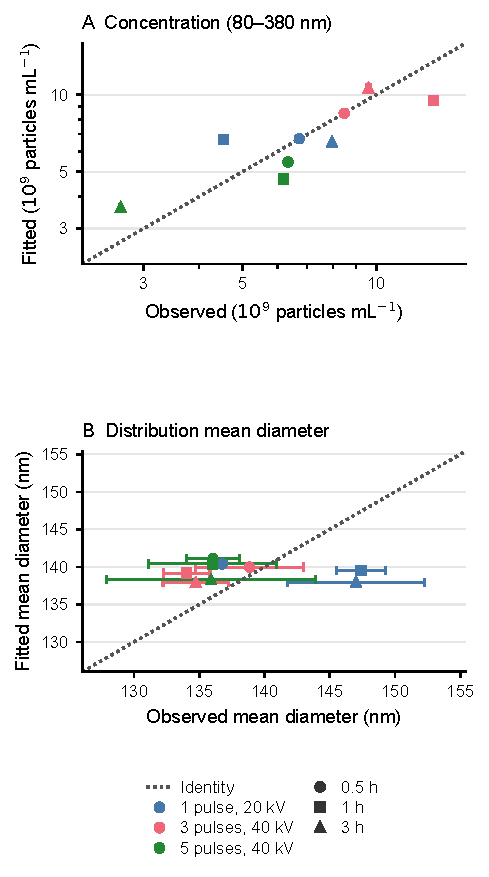
\includegraphics[width=0.72\textwidth]{figure4_calibration.pdf}
\caption{\textbf{The selected observation model reproduces aggregate concentration and mean diameter in sample.} a, Fitted and observed particle concentration integrated over 80--380 nm. b, Fitted and observed whole-histogram mean diameter. Dotted lines indicate identity; horizontal bars show observed sample standard deviations. Colours denote pulse-labelled conditions and symbols denote harvest times. The comparisons use the same observations used for fitting and therefore do not measure out-of-sample prediction.}
\label{fig:calibration}
\end{figure}

\subsection*{Sensitivity separates influential processes from locally constrained parameters}

Morris screening linked simulated extracellular concentration at 3 h primarily to pathway-to-particle source conversion, basal medium/large-EV production and extracellular disappearance (Fig.~\ref{fig:sensitivity}). The largest mean absolute elementary effects in the mechanistic analysis were 0.420 for source conversion, 0.401 for basal medium/large-EV release and 0.401 for the basal budding pool. Effective loss, scission, degradation, uptake and adsorption followed with values between 0.347 and 0.380. The signs of elementary effects agreed with their modeled roles: source and release terms increased concentration, whereas disappearance terms decreased it.

In the observation layer, medium/large- and small-EV source scales had mean absolute elementary effects of 12.98 and 9.34 for the reference condition at 3 h, compared with 2.38 for effective half-life. The empirical gain coefficients were insensitive at the centered reference condition by construction but influential in other conditions. These rankings depend on the provisional ranges and output transformations and should not be interpreted as an experimentally established hierarchy.

Local residual-curvature analysis gave a condition number of $6.3\times10^{21}$, with singular values spanning approximately 22.8 to $2.8\times10^{-10}$. All four apoptotic-body-associated parameters had near-zero local information, consistent with their unstable fitted values. Broad-range sensitivity and local constraint therefore described different properties: a parameter could change the output over a wide range while remaining unconstrained near the selected fit. Conditional Sobol estimates, target-specific sensitivity maps and local-information diagnostics are provided in Supplementary Figs.~9--11.

The combined analysis identified three measurement priorities. Orthogonal particle and pathway-associated measurements are required to separate conversion and recovery from biological release. Additional harvests between 1 and 3 h, accompanied by time-matched sham samples, would distinguish continuing production from extracellular disappearance. Finally, confirmed field dosimetry together with early calcium and injury measurements would test whether the empirical exposure gain can be replaced by an upstream mechanism. The corresponding decision summary is shown in Supplementary Fig.~12.

\begin{figure}[htbp]
\centering
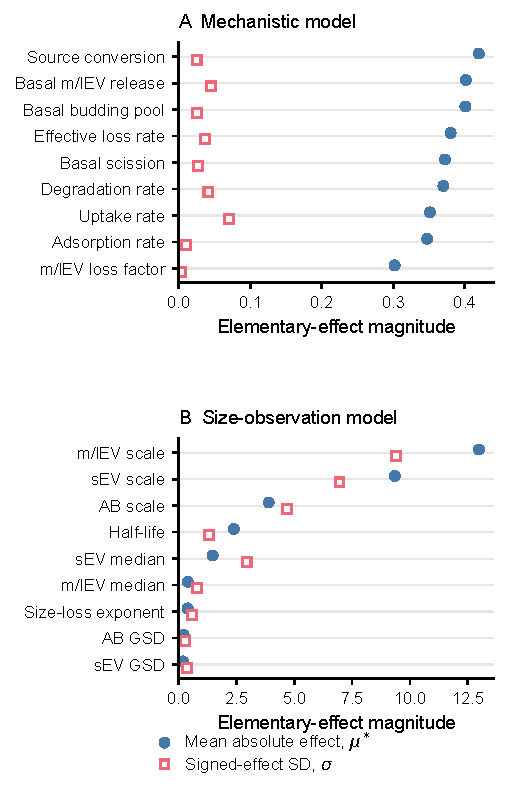
\includegraphics[width=0.78\textwidth]{figure5_sensitivity.pdf}
\caption{\textbf{Parameter influence depends on whether mechanistic or observational output is considered.} a, Morris mean absolute elementary effects for mechanistic extracellular concentration at 3 h. b, Effects for concentration inside the observed 80--380-nm window with upstream trajectories fixed. Circles show mean absolute elementary effects and open squares show the sample standard deviation of signed effects. The mechanistic and observation analyses used different parameter domains and ranges; horizontal magnitudes are therefore not comparable between panels. Two trajectories were used per mechanistic parameter and four per observation parameter. AB, apoptotic body; EV, extracellular vesicle; GSD, geometric standard deviation; m/lEV, medium/large EV; sEV, small EV.}
\label{fig:sensitivity}
\end{figure}

\section*{Discussion}

This study establishes a computational connection between a nanosecond electrical perturbation and an extracellular particle population measured hours later. The principal result is not a single optimized protocol, but a separation of processes that are otherwise confounded in concentration data: electrical exposure and membrane charging, calcium and bioenergetic responses, remodeling and repair, pathway-resolved vesicle release, extracellular disappearance and measurement. This separation allowed the model to reproduce the dominant measured particle-size distribution while making its unresolved dose dependence and weakly constrained particle classes explicit.

The model is consistent with a growing experimental picture in which electrical and calcium signals regulate membrane trafficking at several levels. Direct-current electric fields can increase small-EV secretion through ceramide-dependent budding and increased intraluminal-vesicle formation \cite{huang2026electric}. Although that exposure differs substantially from nsPEF stimulation, it supports the broader premise that membrane polarization can regulate vesiculogenesis. The nsPEF study most closely aligned with our upstream layers found size-dependent permeability, calcium-dependent resealing, osmotic swelling and stiffness loss \cite{kielbik2026selective}. These observations support representing cell geometry and repair capacity as determinants of response rather than treating nominal pulse settings as a transferable dose.

Calcium provides a plausible link between transient permeability and longer-lived vesicle release. Extracellular ATP stimulates both small- and large-EV secretion through P2X7-associated calcium entry in several cancer cell lines \cite{kao2023atp}. Calcium-activated scrambling changes the exposed membrane proteome within minutes \cite{tuomivaara2024slapshot}, and TMEM16E-dependent phosphatidylserine exposure can recruit a compensatory macropinocytic repair response \cite{kim2025tmem16e}. In the present simulations, calcium-dependent remodeling increased budding competence, whereas repair limited progression toward injury-associated output. These relationships are mechanistically plausible but are not yet jointly calibrated in the producer cells used for the particle measurements. Their current value is to define measurements that can distinguish competing explanations.

The fitted observation model reinforces the need to separate biogenesis pathways from operational diameter classes. Distinct extracellular particles can overlap in diameter and composition, and secreted midbody remnants provide an example of a particle class molecularly distinct from both exosomes and plasma-membrane microparticles \cite{peterman2021midbody}. The fitted small- and medium/large-EV medians should consequently be interpreted as effective pathway kernels, not direct identification of exosomes or microvesicles. The near-zero apoptotic-body contribution is likewise not evidence that these particles were absent; the measured window and the available time points supplied little information about that pathway.

The inferred effective half-life summarizes several extracellular processes rather than a molecular degradation constant. Uptake, degradation, adsorption, aggregation, sampling and isolation can all reduce measured concentration. The present data did not allow those processes to be estimated separately. The strong sensitivity to source conversion and extracellular disappearance therefore identifies an experimental ambiguity: an apparent concentration decline can be explained by altered production, altered loss or both. Time-matched sham samples, recovery controls and orthogonal particle assays are needed before assigning the fitted loss to a specific biological process.

The empirical exposure gain improved the fit but marks a limitation of the mechanistic model. Because delivered field, electrode separation, waveform, temperature and complete culture metadata remain unconfirmed, the source labels cannot calibrate membrane voltage or absorbed energy. The gain currently absorbs differences that may arise from dosimetry, viable-cell number, recovery, dilution, instrument response or missing biology. Retaining it as an explicit observation-layer term prevents these effects from being silently incorporated into calcium or vesicle-biogenesis constants. A decisive next test is to replace the gain with measured exposure and early cellular responses and evaluate performance on held-out pulse conditions.

Several additional limitations define the present domain of interpretation. The intracellular equations are reduced and contain provisional constants; acute nanosecond dynamics are compressed into pulse descriptors rather than directly integrated. The model represents a typical producer cell and does not yet propagate population heterogeneity. Repeated-measurement independence, instrument detection limits and the origin of the sham measurements require confirmation. The calibration is in-sample, and the sensitivity designs are screening analyses rather than converged uncertainty quantification. Cargo and potency modules are implemented as interfaces but were not constrained by the present dataset. These limitations preclude claims of biological parameter identification or prospective optimization.

The analysis nevertheless yields a falsifiable experimental program. Measurements of delivered field and temperature define the physical input; early permeability, calcium, phosphatidylserine and viability measurements constrain the transition from exposure to remodeling; pathway-associated markers and electron or imaging-flow methods constrain particle identity; and denser extracellular time courses separate production from disappearance. Because each measurement maps to a defined model interface, negative or discordant results can revise a specific mechanism without discarding the complete pipeline. In this way, the model provides a structured route from bioelectric exposure to EV manufacturing questions while preserving the distinction between simulated mechanism, fitted observation and biological evidence.

\section*{Methods}

\subsection*{Model design}

The model was implemented as a sequence of coupled modules spanning pulse delivery, membrane and organelle electrodynamics, ion transport and bioenergetics, remodeling and repair, EV-biogenesis pathways, extracellular particle kinetics and measurement. Each module exposes a defined set of inputs and outputs so that reduced equations can be replaced without changing the complete analysis interface. Simulations were performed with the \texttt{electro\_exocytosis} Python package. The repository records merged parameter values and run metadata for each scenario.

Nanosecond pulses were represented by amplitude, width, number, repetition rate and waveform descriptors. The electrical pulse was not integrated on the downstream seconds-to-hours time grid. Instead, waveform- and geometry-dependent descriptors initialized or forced the reduced electrodynamic model. A first-order charging relation represented the plasma membrane,
\begin{equation}
C_{\mathrm m}\frac{\mathrm d\Delta V_{\mathrm m}}{\mathrm dt}+G_{\mathrm m}(t)\Delta V_{\mathrm m}=f(E(t),\theta),
\end{equation}
where $C_{\mathrm m}$ is membrane capacitance, $G_{\mathrm m}$ is effective conductance, $\Delta V_{\mathrm m}$ is induced transmembrane voltage and $\theta$ contains geometry and material parameters. Related reduced states represented organelle charging and permeability. Pulse-energy calculations included a waveform-aware Joule estimate,
\begin{align}
\chi_{w}&=\frac{1}{t_{p}}\int_{0}^{t_{p}}\left[\frac{E(t)}{E_{\mathrm{peak}}}\right]^2\mathrm dt,\\
u_{J}&=\sigma E_{\mathrm{peak}}^2t_{p}N\chi_{w}\langle g_E^2\rangle,
\end{align}
where $\sigma$ is medium conductivity, $t_p$ is pulse width, $N$ is pulse number and $\langle g_E^2\rangle$ is a geometry factor. These quantities are model descriptors and were not equated with measured temperature.

\subsection*{Ion transport, remodeling and repair}

Electroporation-dependent permeabilities supplied ionic fluxes to compartmental balance equations. The calcium balance included pore-mediated entry, plasma-membrane transport, endoplasmic-reticulum release and uptake, mitochondrial exchange and buffering. Sodium, potassium and chloride states contributed to osmotic stress. Reduced mitochondrial-potential, reactive-oxygen and adenosine-triphosphate states represented bioenergetic response and recovery. Model time was expressed in seconds internally and reported in seconds or hours according to the process shown.

Submembrane calcium activated phosphatidylserine exposure, calpain, annexin-associated repair, lysosomal repair and actin remodeling through saturating response functions. A generic activation state was
\begin{equation}
A_x=\frac{C_{\mathrm{sub}}^{n_x}}{K_x^{n_x}+C_{\mathrm{sub}}^{n_x}},
\end{equation}
where $C_{\mathrm{sub}}$ is the submembrane calcium state, $K_x$ is its half-activation scale and $n_x$ is a Hill coefficient. Damage increased with residual permeability and oxidative stress and decreased with the repair state. These equations are reduced phenomenological representations rather than molecularly resolved reaction networks.

\subsection*{Pathway-resolved vesicle release}

Small-EV release was represented by multivesicular-body maturation, intraluminal-vesicle loading, docking and calcium-dependent fusion. Medium/large-EV release was represented by a plasma-membrane budding pool regulated by phosphatidylserine and actomyosin states. A separate injury-linked state generated apoptotic-body output. The total release rate was
\begin{equation}
R_{\mathrm{EV}}(t)=R_{\mathrm{sEV}}(t)+R_{\mathrm{m/lEV}}(t)+R_{\mathrm{AB}}(t).
\end{equation}
Release was propagated together with a time-varying viable-producer fraction. Simulations used non-negative states and parameter constraints. The scenario files and complete parameter snapshots accompanying the code define all constants used for the reported runs.

\subsection*{In vitro particle-size measurements}

Size-resolved extracellular particle measurements were obtained from CD4$^+$ cell preparations nominally containing $5\times10^6$ cells per batch. The supplied export contained conditions labelled as one pulse at 20 kV, three pulses at 40 kV and five pulses at 40 kV, sampled at 0.5, 1 and 3 h. Complete delivered-field, electrode, culture, harvest, dilution, recovery and instrument metadata were not available. The numerical voltage values were therefore retained as source labels and not interpreted as kV cm$^{-1}$.

Particle concentrations were rebinned into 15 common 20-nm bands spanning 80--380 nm before arithmetic means and sample standard deviations were calculated. The analysis included 26 stimulated histograms, with three repeated measurements per condition and time except for the three-pulse, 40-kV-labelled condition at 1 h ($n=2$). Three undated cell-containing sham histograms were averaged to provide a provisional initial extracellular distribution. Three separately labelled undated ``sham media'' histograms were excluded because their relationship to the cell-containing controls was unresolved. The independence of repeated measurements was not established; they were not treated as independent biological replicates for inferential statistics.

\subsection*{Experimental-to-computational scaling}

The observation bridge used $5\times10^6$ initial cells and a provisional medium volume of 5 mL, equivalent to $10^6$ initial cells mL$^{-1}$. No measured viability trajectory was available. Recovery and dilution were set to one, while the viable-cell factor followed the simulated producer-cell trajectory. These are interface assumptions, and fitted pathway-to-particle conversion factors absorb their uncertainty.

For release pathway $q$, increments in cumulative output were distributed through a non-negative lognormal kernel. The median was allowed to depend on a matched upstream state,
\begin{equation}
d_{50,q}(t)=d_{50,q}^{0}\exp[\gamma_qS_q(t)],
\end{equation}
where $d_{50,q}^{0}$ is the baseline median, $\gamma_q$ is a coupling coefficient and $S_q(t)$ is the exposed-minus-reference upstream state. Pathway identity was preserved even when operational size distributions overlapped.

Extracellular concentration $C_b$ in latent diameter band $b$ followed
\begin{equation}
\frac{\mathrm dC_b}{\mathrm dt}=\rho_v(t)\sum_q a_qK_{qb}(t)r_q(t)-\frac{\ln2}{t_{1/2,150}}\left(\frac{d_b}{150\,\mathrm{nm}}\right)^\eta C_b,
\end{equation}
where $\rho_v$ is viable producer-cell density, $a_q$ converts pathway units to particles, $K_{qb}$ is kernel mass, $r_q$ is the pathway release rate, $t_{1/2,150}$ is effective half-life at 150 nm and $\eta$ defines size dependence. Initial and newly released particles experienced the same loss. An explicit matrix mapped latent stocks to the measured bands. In the absence of instrument-response calibration, this matrix was identity-like inside 80--380 nm, with no broadening, unit recovery and zero background.

\subsection*{Calibration and model comparison}

Calibration treated integrated concentration and normalized size composition separately. For condition $c$, time $t$ and band $b$, residuals were
\begin{equation}
r^{\mathrm{total}}_{ct}=\ln\left(\frac{\widehat T_{ct}}{T_{ct}}\right),\qquad
r^{\mathrm{size}}_{ctb}=\sqrt{\widehat f_{ctb}}-\sqrt{f_{ctb}},
\end{equation}
where $T$ is total concentration in the measured window and $f$ is the corresponding band fraction. Sample standard deviations were used for descriptive figures but not as inverse-variance weights because there were only two or three repeated measurements and bands from each histogram were correlated.

We compared time-invariant kernels, state-conditioned kernels and state-conditioned kernels with a shared empirical exposure gain,
\begin{equation}
g_c=\exp[\beta_1(D_c-0.72)+\beta_2(D_c-0.72)^2],
\end{equation}
where $D_c$ is the model-derived dose index and 0.72 is a fixed centering value. Each variant was fitted by bounded nonlinear least squares from 24 starting vectors: one canonical vector and 23 seeded Latin-hypercube points. A weak penalty of weight 0.25 regularized pathway medians and widths, the size-loss exponent, state couplings and empirical gain coefficients toward their initial values. The composite penalized score was used descriptively because the residuals were not derived from a complete sampling likelihood.

Fit summaries included log$_{10}$ concentration root-mean-square error and its multiplicative equivalent, percentage errors, Hellinger and Wasserstein distances between size distributions, and absolute error in mean diameter. Optimization endpoints within 1\% of the lowest regularized objective were summarized to assess numerical stability. These ranges are not confidence intervals or estimates of biological variability.

\subsection*{Global sensitivity analysis}

Morris screening was performed separately for runtime-mechanistic and observation-layer parameters \cite{morris1991factorial}. The mechanistic analysis varied 198 consumed runtime parameters for the three-pulse, 40-kV-labelled scenario. The observation analysis fixed upstream trajectories and varied the 16 fitted observation parameters. Runtime parameters were sampled over provisional default-centered ranges, generally 0.8--1.2 times positive defaults. Observation parameters were sampled across optimizer bounds in their fitted coordinates. These domains have different widths and transformations and their sensitivity magnitudes were not compared directly.

Morris elementary effects used six levels and a normalized step magnitude of 0.6. Two trajectories were generated for each mechanistic parameter and four for each observation parameter. We reported the mean absolute elementary effect and the sample standard deviation of signed effects. A second, conditional analysis selected seven mechanistic and eight observation parameters using their largest screened effect over configured targets. Independent inputs were sampled with scrambled Sobol sequences using 64 base rows. First- and total-order indices used Saltelli and Jansen estimators, respectively \cite{saltelli2010variance,jansen1999analysis}. Two hundred paired-row resamples supplied descriptive intervals. The small designs were used for screening and do not establish convergence.

\subsection*{Local information and measurement-priority analyses}

The selected fit's unregularized residual vector was differentiated numerically with respect to optimization coordinates. Bound-aware central differences used steps of $10^{-4}\max(|x_i|,u_i-l_i,1)$. With $D_{ii}=\max(|x_i|,0.1(u_i-l_i))$, the scaled residual-curvature matrix was
\begin{equation}
G=(JD)^{\mathsf T}(JD).
\end{equation}
A relative singular-value cutoff of $10^{-10}$ was applied to its generalized inverse. Because the residuals are not based on a calibrated observation likelihood, $G$ was interpreted as a local geometric diagnostic, not a Fisher information matrix. It does not provide confidence intervals or establish structural identifiability \cite{raue2009structural}.

An exploratory priority score combined normalized sensitivity, assumed uncertainty, a local information-gap proxy, measurability and feasibility using a weighted geometric mean. Equal weights were compared with doubled measurement/feasibility weights and doubled sensitivity/information-gap weights. Measurability and feasibility values were assigned heuristically; the resulting ranking is a decision aid rather than formal optimal experimental design.

\subsection*{Statistics and reproducibility}

No null-hypothesis significance tests were applied to the particle dataset because biological independence and the sampling hierarchy were unresolved. Observations are shown as arithmetic mean $\pm$ sample standard deviation, with $n$ defined as the number of supplied repeated histograms. All 24 calibration starts completed. Random seeds, optimizer bounds, sampled parameter ranges, parameter registries and source values for sensitivity figures are retained with the analysis. The model code records parameter snapshots and run metadata to support computational reproduction. No randomization or blinding was applicable to the computational analyses; the experimental randomization and blinding status was not available in the supplied metadata.

\section*{Data availability}

The processed particle distributions, calibration summaries and sensitivity-analysis tables supporting this draft are retained with the analysis repository. Source data underlying each submitted graph should be deposited in a persistent public repository before submission; accession information will replace this sentence. Raw experimental files and complete acquisition metadata remain under the control of the experimental study team and their availability must be confirmed before submission.

\section*{Code availability}

The custom Python package, scenario files and analysis scripts used for the simulations are contained in the \texttt{electroexo} repository. A versioned public release and persistent archive identifier are required before submission. The release should include the exact parameter snapshots, random seeds and commands associated with each main and supplementary figure.

\section*{Acknowledgements}

[Add essential acknowledgements and all funding information. Communications Biology does not use a separate Funding section.]

\section*{Author contributions}

[Replace with a contribution statement that identifies the specific work of A.G., M.M. and R.M.L.C.-B. and disambiguates all initials.]

\section*{Competing interests}

The authors declare no competing interests.

\section*{Additional information}

Supplementary information accompanies this paper.


\bibliographystyle{unsrtnat}
\bibliography{references/references}
\end{document}
